\Chapter{Az adatbázismotor felépítése és működése}

\section{Java implementáció}

A \textit{Java} nyelvnek számos olyan előnye van, ami miatt jó választásnak bizonyult egy adatbázismotor elkészítéséhez. Ilyen például, hogy
\begin{itemize}
\item a nyelv platformfüggetlen. A program átvihetőségével kapcsolatos problémák így gyakorlatilag megoldottnak tekinthetők.
\item Gazdag eszközkészletet biztosít.
\item A virtuális gép implementációja kellőképpen hatékony ahhoz, hogy a lekérdezéseket időben végre lehessen hajtani.
\item Korábban már voltak jó tapasztalataim a Java nyelvvel és környezetével kapcsolatban.
\end{itemize}

Az elsődlegesen megoldandó problémát a térképadatok tárolása jelentette. Az adatok tényleges tárolásához több lehetőség is adott volt.
\begin{itemize}
\item Kidolgozható egy olyan, saját fájlformátum, amely kifejezetten térképadatok hatékony tárolására van specializálva.
\item A térképadatok kezelésének egy lehetséges módja, hogy azokat egy, már létező adatbázis modelljére képezzük le. Ezzel az adott adatbázismotort, mint kész komponenst lehet alkalmazni.
\item Az adatok strukturált tárolását XML és JSON formátumok segítségével elegánsan meg lehet oldani.
\end{itemize}

A saját fájlformátum kidolgozására, és így a tárolás alacsony szintű megvalósítására azért nem került sor, mert egyelőre annak a belátása a cél, hogy a térképadatbázis funkcióira a gyakorlatban valóban szükség van. A hatékonyság itt tehát még elsősorban a fejlesztők munkáját illetően jelenik meg, nem pedig a futási időkben és a tárigényben.

Egy létező adatbázismotornak a használata az alkalmazásoknak egy plusz külső függőséget jelentene. Az SQLite tünhet még egy szerencsés választásnak ilyen esetben, mivel az függvénykönyvtárként használható. A kialakított objektum-orientált adatbázis modell relációs modellre való leképzése természetesen megoldható lett volna, viszont a fejlesztés közben mutatkozott annál hatékonyabb megoldás.

Az XML és JSON nyelvek egyaránt alkalmasak a térkép, és a rajta lévő entitások jellemzőinek tárolásához. A JSON azért bizonyult jobb választásnak, mert az adatmodellje közelebb áll a térképadatbázis modelljéhez, feldolgozása egyszerűen megoldható és tárigényben is kisebb költséget jelent.

\section{Az adatbázismotor és a driver kapcsolata}

\begin{figure}[htb]
	\begin{center}
		\includegraphics[scale=0.1]{images/database}
		\caption{A komponensek együttműködés}
		\label{fig:database}
	\end{center}
\end{figure}

Az adatbázismotor közvetlenül nem tud kommunikálni a kliens programmal. Ehhez szükség van egy közbülső, aktív szoftveres kapcsolóelemre, amelyet meghajtóprogramnak, vagy angol terminológia szerint \textit{driver}-nek szoktak nevezni.

Az adatbázis motor és a driver között a kommunikáció (\textit{az adatok tárolási módjához hasonlóan}) JSON alapú. Ez lehetővé teszi, hogy a driver és az adatbázismotor más nyelven legyen implementálva. Számítógépes játékokat implementálhatnak például C, C++, C\#, Java nyelveken, és ahhoz, hogy mindegyikkel kompatibilis legyen az adatbázismotor, ahhoz rosszabb esetben arra lenne szükség, hogy a motort minden nyelven implementáljuk. Ez komoly fejlesztőmunkát igényelne, e helyett csak egy drivert kell implementálni ezen nyelvekhez, amely kommunikál az adatbázis motorral. A projektre nézve a későbbiekben nem csak Java nyelven írt drivert szeretnénk, hanem C++ és C\# is a tervek között van.

\subsection{Lekérdezések kiértékelése}

A \ref{fig:database}. ábrán szemléltetjük a lekérdezés feldolgozásának és kiértékelésének folyamatát. A kliens a driveren keresztül kiad egy \texttt{executeQuery(String query)} hívást, amelyben a lekérdezés az egy karakterlánc. Ez adódik át a \textit{Parser} nevű, nyelvi értelmező komponensnek. Az adatbázismotor \textit{Parser} komponense a lekérdezésobjektumokat a \texttt{Builder} osztályok metódusaival építi fel. Ezt követően az előállított lekérdezés objektumnak meghívódik az \texttt{execute} metódusa, és ennek eredménye \texttt{SELECT} esetén egy lista amely objektumokat tartalmaz. Ezt a listát a motor átadja a \textit{JSON Serializer} komponensnek, ami előállítja ebből a listából a JSON-t, amit továbbít a drivernek, aminek a \textit{JSON Deserializer} komponense foglya feldolgozni, és előállít belőle egy eredmény listát. A driver a kliens program számára már értelmezhető formában adja vissza az eredmény listát. Ez a körfolyamat játszódik le minden lekérdezés esetén.

\subsection{Az ütközésvizsgálat megvalósítása}

\begin{figure}[htb]
\begin{center}
    \includegraphics[scale=0.15]{images/collision}
    \caption{Ütközés vizsgálat két alakzat között}
    \label{fig:collision}
\end{center}
\end{figure}

A lekérdezések közül gyakorlati szempontból az egyik legfontosabb az ütközésvizsgálat.

Az ütközés vizsgálat során általában elegendő azt vizsgálni, hogy két alakzat valamilyen mértékben fedésben van-e egymással. Az ütközés vizsgálatnak itt viszont van egy másik fajtája is, amikor mozogni szeretnék egy entitással, és azt szeretnénk megvizsgálni, hogy egyik pontból a másikba mozogva ütközik-e valamely adatbázisban tárolt elemmel.

Az ütközési problémának sajnos nincs minden esetben megoldása, és ha van, akkor sem feltétlenül egyértelmű. Itt implementálásra került egy olyan kiegészítő módszer, amellyel egy jó közelítést lehet adni, hogy az ütközést követően hova kerülne az objektum. Valós időben vizsgálva az objektumok mozgását ez egyfajta \textit{csúszós hatás}t kelt. Az adatbázis ki tudja úgy számolni az új pozícióját egy objektumnak, hogy a felhasználó csak azt adta meg, hogy melyik pozícióba szeretné mozgatni az elemet.

A \ref{fig:collision}. ábrán látható, hogy milyen elven oldottam meg a problémát. A bal fels\H o sarokban lév\H o zöld téglalap az entitás, amivel mozogni szeretnék. Minden entitást egy bal fels\H o sarok koordinátával és egy szélesség-magasság egész értékekkel lehet meghatározni az ütközésvizsgálat szempontjából. A bal fels\H o sarkából kiinduló egyenes köti össze a bal fels\H o sarkát azzal a ponttal, ahová mozogni szeretne az entitás. A jobb alsó sarokban lév\H o téglalap ez az objektum, amivel ütközést vizsgálok. Látható, hogy a bal fels\H o sarkához hozzátoltam a mozogni szándékozó entitást, és így kaptam egy nagyobb téglalapot.
Az új téglalap négy határoló egyenesével megvizsgálom, hogy van-e metszéspontja annak az egyenesnek, ami az entitás bal fels\H o sarkából indul. Ha van, akkor ütközne, ha nincs egyik oldali egyenessel sem metszéspont, akkor az azt jelenti, hogy azzal az objektummal nem ütközik az entitás, ha oda lép. Természetesen ezt az eljárást minden pályaelemre meg kell ismételni.

A \ref{fig:collision2}. ábrán a zöld téglalappal szeretnénk mozogni olyan pontba, ahol ütközne már a nagy piros téglalappal. A sárga téglalap lesz az, ahova lecsúszik majd az ütközést követ\H oen a zöld entitás.

\begin{figure}[htb]
	\begin{center}
		\includegraphics[scale=0.15]{images/collision2.png}
		\caption{Két alakzat ütközésének következménye}
		\label{fig:collision2}
	\end{center}
\end{figure}

\subsection{Két egyenes metszéspontjának kiszámítása}

Az implementáció sokkal egyszerűbbnek bizonyult homogén koordináta rendszerben, mint Descartes-ban. Homogén koordináta rendszerben a pont és az egyenes felírási módja megegyezik, így a két pontra felírható egyenes, és két egyenes metszéspontja is ugyanazzal a művelettel számolható \cite{Banya5}.

A két pontra illeszkedő egyenes egyenlete homogén koordináta rendszerben a következőképpen néz ki.
$$
e = (
\begin{matrix}
a, & b, & c \\
\end{matrix}
) =
\left(
\begin{matrix}
i & j & k \\
a_1 & a_2 & 1 \\
b_1 & b_2 & 1 \\
\end{matrix}
\right) =
(
\begin{matrix}
a_2 - b_2, & b_1 - a_1, & a_1 b_2 - b_1 a_2
\end{matrix}
)
$$
Két egyenes metszéspontjának a következőképpen határozhatjuk meg.
$$
P = (
\begin{matrix}
p_1, & p_2, & p_3 \\
\end{matrix}
) =
\left(
\begin{matrix}
i & j & k \\
a & b & c \\
e & f & g \\
\end{matrix}
\right) =
(
\begin{matrix}
bg - fc, & ec - ag, & af - eb
\end{matrix}
)
$$
A $P$ pont Descartes koordinátái ez alapján
$$
x = \dfrac{bg - fc}{af - eb}, \quad
y = \dfrac{ec - ag}{af - eb}
$$

\subsection{Interfész az ütközésvizsgálathoz}

Az alkalmazás a \texttt{Collision} interfészen keresztül veheti igénybe az ütközés vizsgálattal kapcsolatos funkciókat. Ez foglalja magába az előzőekben bemutatott homogén koordinátás számítás implementációt.

Az ütközésvizsgálatra nézzük az alábbi példát!
\begin{sql}
UPDATE azeroth MOVE mine TO Point(10,10) WHERE mine.id = 11; 
\end{sql}
A fenti lekérdezés azokat az objektumokat mozgatja el a $(10, 10)$ pontba, amelyeknek van \texttt{id} attribútuma, és annak értéke 11. Ebben az esetben ütközést vizsgálva mozgat, tehát egyáltalán nem biztos, hogy a lekérdezés eredménye az lesz, hogy a feltételre megfelelő objektumok a $(10, 10)$ pontba kerülnek, mert előfordulhat, hogy ütköznek, és abban az esetben az adatbázismotor számol nekik új pozíciót.

A mozgatás elvégeztethetjük csak az egyik koordinátára is, például az
\begin{sql}
UPDATE azeroth MOVE mine.x TO 10 WHERE mine.id = 11;
\end{sql}
lekérdezés csak az $x$ tengely szerinti mozgatást érinti.

\section{Lekérdezés objektumok}

Az adatbázismotorhoz a beérkező lekérdezés szöveges formában kerül át. Ennek a következő lépéseken kell keresztül mennie, hogy az adatbázisban végrehajtásra kerüljön.
\begin{itemize}
\item A szöveget a \textit{Tokenizer} komponens tokenekre bontja.
\item A \textit{Parser} komponens a \texttt{Builder} osztályok használatával lekérdezésobjektumot készít belőle.
\item A lekérdezés objektumnak meg kell hívni az \texttt{execute} metódusát a lekérdezés végrehajtásához.
\end{itemize}

Az átalakítás során számos szintaktikai vagy szemantikai hiba előfordulhat. Ezeket a nyelvi feldolgozás és a végrehajtás során is kivételobjektumok dobásával jelzi a hibát detektáló kódrész.

Ez minden lekérdezéstípus esetében így történik. A következőkben az egyes lekérdezéstípusok kerülnek bemutatásra ennek megfelelően. A példákon keresztül láthatjuk majd, hogy hogyan néz ki az említett \texttt{Builder} osztályok interfésze.

\subsection{A SELECT lekérdezés objektum}

Az implementáció szempontjából a \texttt{WHERE} kulcsszó után szereplő kifejezés ábrázolása bizonyult összetettebb feladatnak. Egy ilyen lekérdezés egyszerűbb változata például az alábbi.
\begin{sql}
SELECT mine FROM azeroth WHERE mine.x = 10 AND mine.y < 20;
\end{sql}

A \texttt{WHERE} kulcsszó után szereplő feltételben tetszőleges sok állítás szerepelhet logikai műveletekkel összekapcsolva és különféle módokon zárójelezve. Ennek az ábrázoláshoz a megoldást egy bináris fa jelentette.

Amennyiben a feltételeket fa struktúrába sikerül rendezni, akkor kiértékeléskor elegendő \textit{postorder} bejárással végigiterálnunk a fa elemein, ahogy a \ref{fig:postorder}. ábrán látható.

A fa levelein találhatóak az operandusok, a csomópontjaiban pedig a bináris logikai operátorok. Egy csomópont kiértékelésekor így mindig egy logikai kifejezést kapunk.

A \texttt{SELECT} lekérdezés kiértékelése ennek segítségével úgy történik, hogy a feltételt megvizsgáljuk a szóbajöhető objektumokra, és amelyikre igaz, az belekerül az eredmény listába.

\begin{figure}[htb]
	\begin{center}
		\includegraphics[scale=0.1]{images/postorder}
		\caption{\texttt{WHERE} feltétel kiértékelése \textit{postorder} fabejárással}
		\label{fig:postorder}
	\end{center}
\end{figure}

\subsection{A \texttt{WHERE} utáni kifejezés ábrázolása}

A \texttt{WHERE} kifejezés a \texttt{SELECT}, \texttt{UPDATE} és \texttt{DELETE} lekérdezésekben is szerepelhet. A \texttt{WHERE}-ben szereplő kifejezést a későbbi kiértékeléshez gráfként kell ábrázolni. Például tekintsük az alábbi kifejezést!
\begin{sql}
WHERE ((mine.x < 10 AND mine IS Mine)
  OR (mine.location.x = 10 OR mine.y = 20)) AND mine.id = 10;
\end{sql}

A lekérdezés a nyelvi feldolgozás ezen fázisában már tokenek alapján történik. A lekérdezés objektumot egy \texttt{WhereBuilder} típusú objektum fogja felépíteni. A nyelvtani elemző a szintaxis diagramoknak megfelelően bejárja, és ellenőrzi, hogy helyes kifejezésről van-e szó, illetve a megfelelő éleknél meghívja a \texttt{WhereBuilder} metódusait, átadva neki az aktuális token típusát és nevét. A példán keresztül a következőkben láthatjuk, hogy az átalakítás hogyan megy végbe.

A \texttt{WHERE} kulcsszó hatására létrejön egy \texttt{WhereBuilder} objektum.

A nyitózárójeleknél mélyíteni kell a fa mélységén. A részkifejezések, bináris fa lévén, az adott csomópont bal, vagy a jobb gyerekelemébe kerülnek. A builder osztálynak ezért tárolnia kell a fa mélységét, és azt, hogy bal- vagy jobb elem megadása következik-e.

A \texttt{mine.x} esetén a builder létrehoz egy \texttt{Operand} típusú objektumot. Két \texttt{Operand} objektum, és egy \texttt{AND} vagy \texttt{OR} értéket tároló \texttt{Operator}  objektumból a builder létrehoz egy \texttt{WhereLeaf} objektumot. Ez a fa egyik levele lesz. Az aktuális állapotváltozókat figyelembe véve, a mélységi szintet és azt, hogy jobb vagy bal gyerek lesz ez a levél beállítja a builder. A következő metódus meghívásakor az \texttt{AND} logikai operátor adódik hozzá a fához. A builder neki is beállít egy mélységi és egy gyerek értéket. A \texttt{)} karakter észlelése után a buildernek egy olyan metódusa hívódik meg, amely az aktuális mélységi állapotváltozó értékét csökkenti eggyel.

Az említett példán szeretném bemutatni, hogy a fenti algoritmus miként működik. Ennek a lépésnek az alapja, hogy egy listába kerülnek a létrehozott operátorok és operandusok.

\begin{itemize}
\item A \texttt{WHERE} kulcsszó hatására létrejön egy \texttt{WhereBuilder} objektum. A mélységi állapotváltozó értékét 1-re állítja, az aktuális gyerek értéket pedig \texttt{Left} (bal) értékre.
\item A \texttt{(} hatására a mélységi változó értéke kettő lesz.
\item A \texttt{(} hatására a mélységi változó értéke három lesz.
\item A \texttt{mine.x < 10} feldolgozása közben a builder létrehoz egy \texttt{WhereLeaf} levél objektumot, hozzáadva a listához, a mélységi állapotváltozóját négyre állítva. (Levelek esetén nem az aktuális mélységi értéket, hanem azt eggyel megnövelve kell beállítani). A levél aktuális gyerek értékét \texttt{Left}-re állítja, a builder pedig a saját állapotváltozóját \texttt{Right}-ra ezen a szinten. (Ezt egy \texttt{Map} objektummal valósítom meg, ahol a kulcs az, hogy hanyadik szint a fában, az érték pedig a gyerek oldala.) Tehát a builderben a négyes szinthez \texttt{Right} érték lett beállítva.
\item Az \texttt{AND} után a builder létrehoz egy \texttt{Operator} objektumot, a mélységi állapot 3, a gyerek \texttt{Left}-re lesz állítva, majd ezt is hozzáadja a listához.
\end{itemize}

Ez így folytatódik egészen addig, amíg nem ér végig a tokeneken. A feltöltött eredménylista tartalma a lépések végrehajtása utána következő lesz.

\begin{verbatim}
Mélység: 4 gyerek oldal:(false-bal, true- jobb)false mine.x < 10
Mélység: 3 gyerek oldal:(false-bal, true- jobb)false  AND
Mélység: 4 gyerek oldal:(false-bal, true- jobb)true mine IS Mine 
Mélység: 2 gyerek oldal:(false-bal, true- jobb)false  OR
Mélység: 4 gyerek oldal:(false-bal, true- jobb)false mine.location.x 
Mélység: 3 gyerek oldal:(false-bal, true- jobb)true  OR
Mélység: 4 gyerek oldal:(false-bal, true- jobb)true mine.y = 20 
Mélység: 1 gyerek oldal:(false-bal, true- jobb)false  AND
Mélység: 2 gyerek oldal:(false-bal, true- jobb)true mine.id = 10 
\end{verbatim}

Ha ezzel a lépéssel végeztünk, akkor a builder objektum ezt a listát rendezi a mélység és a gyerek oldal attribútumok szerint. A rendezés eredménye a következő.

\begin{verbatim}
Mélység: 1 gyerek oldal:(false-bal, true- jobb)false AND
Mélység: 2 gyerek oldal:(false-bal, true- jobb)false OR
Mélység: 2 gyerek oldal:(false-bal, true- jobb)true mine.id = 10
Mélység: 3 gyerek oldal:(false-bal, true- jobb)false AND
Mélység: 3 gyerek oldal:(false-bal, true- jobb)true OR
Mélység: 4 gyerek oldal:(false-bal, true- jobb)false mine.x < 10
Mélység: 4 gyerek oldal:(false-bal, true- jobb)true mine IS Mine
Mélység: 4 gyerek oldal:(false-bal, true- jobb)false mine.location.x
Mélység: 4 gyerek oldal:(false-bal, true- jobb)true mine.y = 20
\end{verbatim}

\begin{figure}[htb]
	\begin{center}
		\includegraphics[scale=0.1]{images/WhereBuild}
		\caption{A WHERE utáni kifejezésből felépített bináris fa}
		\label{fig:wherePostorderBuilder}
	\end{center}
\end{figure}

\begin{comment}{A fában rosszul szerepel néhány csomópont neve! pl.: 5, mine.location.x}
\end{comment}

Erre a rendezésre azért van szükség, mert így már beszúrási sorrendben vannak az elemek. Ennek a segítségével a fa már egyszerűbben felépíthető.

A fa felépítéséhez végigiterálunk az elemeken és minden csomópontjában beállítjuk sorban a gyerekelemeket. A levél elemekhez értelemszerűen nem kell gyerekelemet rendelnünk. Az eredmény \aref{fig:wherePostorderBuilder}. ábrán látható.

Innentől kezdve rendelkezésünkre áll egy olyan bináris fagráf, amelyet postorder bejárásával a kifejezést az aktuális értékekkel ki tudjuk értékelni.

\subsection{DELETE lekérdezés felépítése}

Tegyük fel, hogy a következő lekérdezés érkezik az adatbázismotorhoz:
\begin{sql}
DELETE mine FROM azeroth WHERE mine.x > 10;
\end{sql}
Mint látható, ez is tartalmaz \texttt{WHERE} kulcsszót, ezért ennek a felépítéséhez is szükségünk lesz majd \texttt{WhereBuilder} objektumra.

A \texttt{DELETE} lekérdezéseket a \texttt{DeleteBuilder} osztály segítségével alakíthatjuk át objektummá.

\begin{figure}[htb]
	\begin{center}
		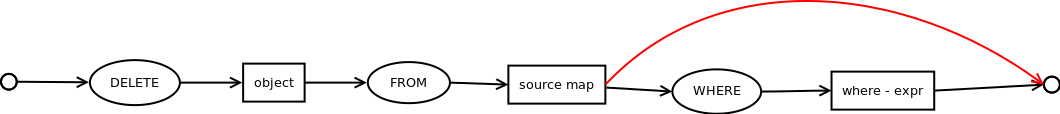
\includegraphics[scale=0.4]{images/delete}
		\caption{A DELETE lekérdezés szintaxis diagramja}
		\label{fig:deleteSytnax}
	\end{center}
\end{figure}

A szintaxis diagram alapján ezek a metódusai hívódnak meg a \texttt{DeleteBuilder} objektumnak:

\begin{java}
DeleteBuilder builder = new Builder();
builder.createDelete("mine");
builder.setFrom("azeroth");
builder.addOperandPiece("mine.x");
builder.addOperator(">");
builder.addOperandPiece("10");
builder.build();
\end{java}

Minden builder osztályban definiáltunk egy \texttt{build} metódust, amely egy \texttt{IQueryObject} példányt ad vissza. Minden lekérdezés objektum implementálja az \texttt{IQueryObject} interfészt, amely egy \texttt{execute} metódust tartalmaz.

\subsection{ALTER lekérdezés felépítése}

Az \texttt{ALTER}, osztályok szerkezetének módosítására szolgáló lekérdezés nyelvi diagramja \aref{fig:alterSytnax} ábrán látható. Tekintsük az alábbi, osztály attribútumának törlésére szolgáló lekérdezést!
\begin{sql}
ALTER CLASS Rectangle DELETEATTRIBUTE x;
\end{sql}

\begin{figure}[htb]
	\begin{center}
		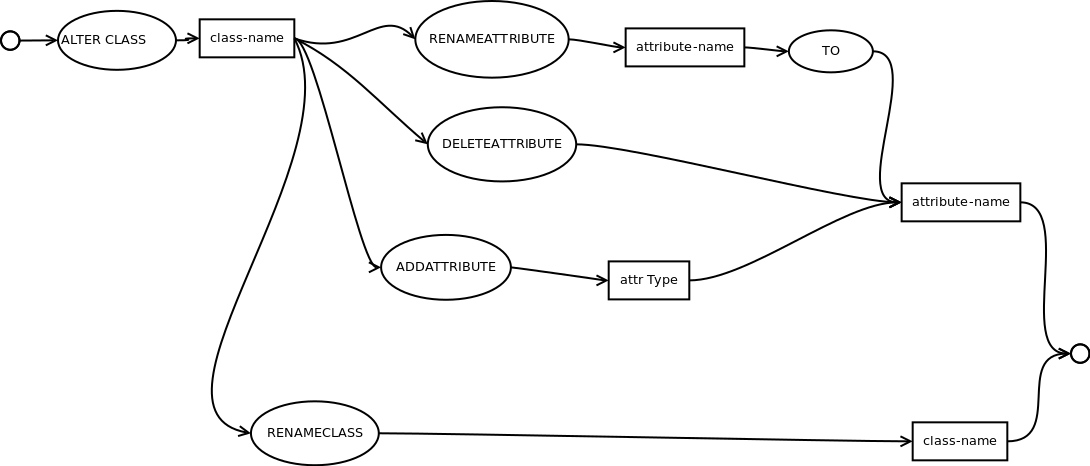
\includegraphics[scale=0.4]{images/alter}
		\caption{Az ALTER lekérdezés szintaxis diagramja}
		\label{fig:alterSytnax}
	\end{center}
\end{figure}

A builder objektum metódusainak használata a fenti lekérdezés esetében:

\begin{java}
AlterBuilder builder = new AlterBuilder();
builder.createAlter("Rectangle");
builder.setAlterType("DELETEATTRIBUTE");
builder.setStringAttribute("x");
builder.build();
\end{java}

Az \texttt{ALTER} lekérdezés 4 altípust definiál, úgy mint

\begin{itemize}
\item osztálynév módosítása
\item attribútum törlése
\item attribútum definiálása
\item attribútum átnevezése.
\end{itemize}

Ezek közül az attribútum létrehozáshoz és átnevezéshez egy plusz attribútumra van szükség, amelyet a \texttt{builder.setOptionalValue} metódussal állíthatunk be a megfelelő attribútum névre vagy típusra.

\subsection{A CREATE lekérdezés felépítése}

A \texttt{CREATE} lekérdezéssel adatbázist, térképet és osztály definíciót lehet létrehozni. Az adatbázisnak és a térképnek a definiálása (\ref{fig:createSytnax}. ábra) az egyszerűbben megvalósítható lekérdezések egyike. Az osztály definiálása (\ref{fig:createClassSytnax}. ábra) ahhoz képest csak néhány további lépést tartalmaz.

\begin{figure}[htb]
	\begin{center}
		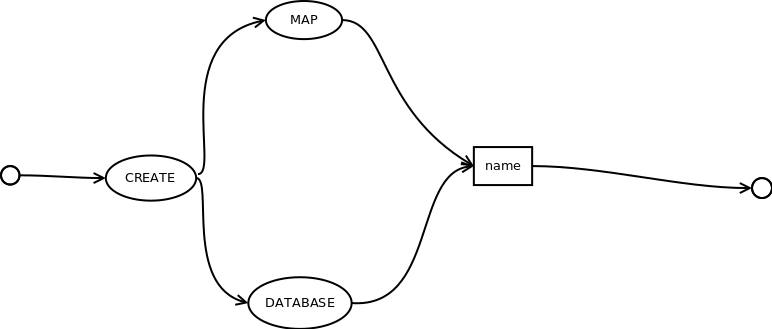
\includegraphics[scale=0.4]{images/create}
		\caption{A \texttt{CREATE} lekérdezés szintaxis diagramja adatbázis és térkép létrehozásra szűkítve}
		\label{fig:createSytnax}
	\end{center}
\end{figure}

\begin{figure}[htb]
	\begin{center}
		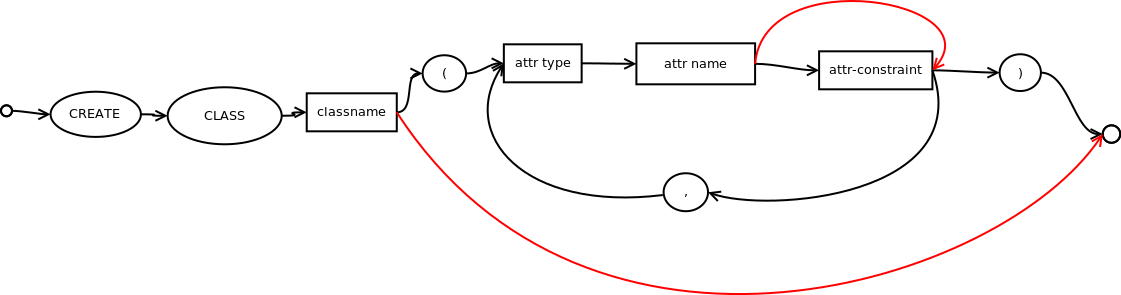
\includegraphics[scale=0.4]{images/createclass}
		\caption{A \texttt{CREATE} lekérdezés szintaxis diagramja osztálydefiníció definiálásához}
		\label{fig:createClassSytnax}
	\end{center}
\end{figure}

Tegyük fel, hogy a következő lekérdezés érkezik az adatbázismotorhoz:
\begin{sql}
CREATE CLASS Harcos(
Number kor,
Number attack DEFAULT 10,
String nev);
\end{sql}

Ennek hatására a \texttt{CreateBuilder} a következő módon fogja létrehozni a lekérdezés objektumot.

\begin{java}
CreateBuilder builder = new CreateBuilder();
builder.setCreateType("CLASS");
builder.setTheCommonValue("Harcos");
builder.addAttributeParam("Number");
builder.addAttributeParam("kor");
builder.insertAttribute();
builder.addAttributeParam("Number");
builder.addAttributeParam("attack");
builder.addAttributeParam("10");
builder.insertAttribute();
builder.addAttributeParam("String");
builder.addAttributeParam("nev");
builder.build();
\end{java}

Az \texttt{insertAttribute} metódus fogja beszúrni az attribútumokat, amely vessző és \texttt{)} karakterek hatására hívódik meg.

\subsection{Az UPDATE lekérdezés felépítése}

Az \texttt{UPDATE} lekérdezés szintaxisa \aref{fig:updateSytnax}. ábrán látható. Vizsgáljuk meg a következő lekérdezést!
\begin{sql}
UPDATE azeroth SET x = 30, y = 40 WHERE mine.id = 10;
\end{sql}

\begin{figure}[htb]
	\begin{center}
		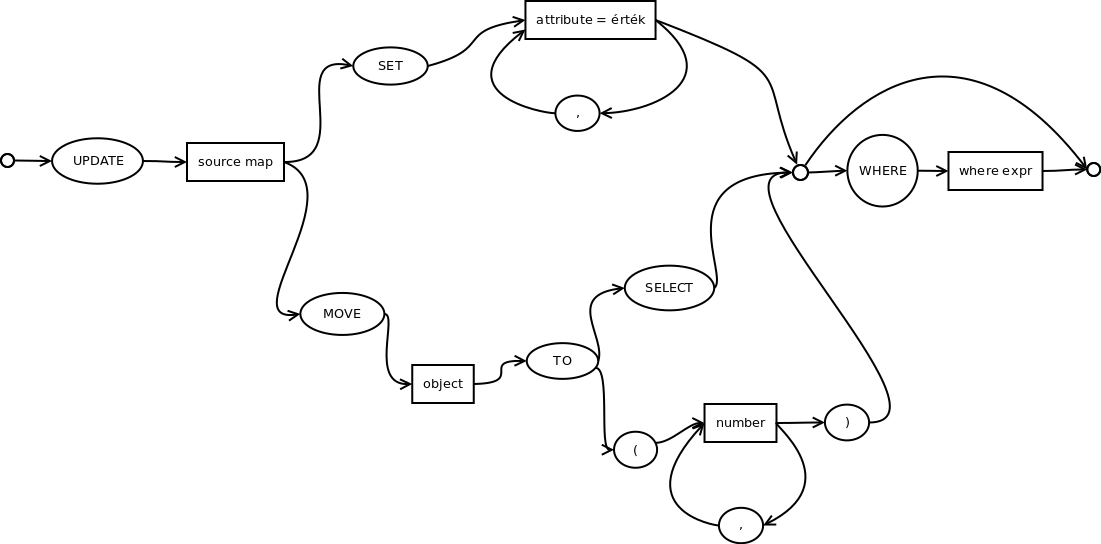
\includegraphics[scale=0.4]{images/update}
		\caption{Az UPDATE lekérdezés szintaxis diagramja}
		\label{fig:updateSytnax}
	\end{center}
\end{figure}

A lekérdezésobjektumot az \texttt{UpdateBuilder} osztály egy példánya fogja felépíteni a következő  metódushívásokat elvégezve.

\begin{java}
UpdateBuilder builder = new UpdateBuilder();
builder.createUpdate("azeroth");
builder.setType("SET");
builder.addSetAttribute("x");
builder.addSetAttributeValue(30);
builder.addSetAttribute("y");
builder.addSetAttributeValue(40);
builder.addOperandPiece("mine.id");
builder.addOperator("=");
builder.addOperandPiece("10");
builder.build();
\end{java}

\subsection{Az INSERT lekérdezés felépítése}

Az \texttt{INSERT} lekérdezés szintaxisdiagramja \aref{fig:insertSytnax}. ábrán látható, a benne szereplő \textit{attrList} és \texttt{valueList} kifejezéseké pedig \aref{fig:attrListSytnax}. és \aref{fig:valueListSytnax} ábrákon.

\begin{figure}[htb]
	\begin{center}
		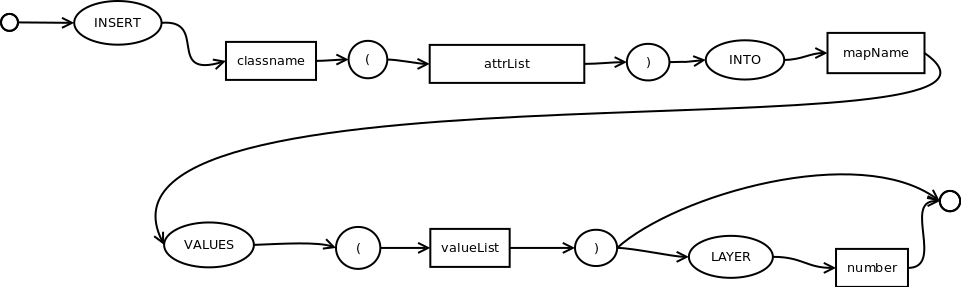
\includegraphics[scale=0.4]{images/insert}
		\caption{Az \texttt{INSERT} lekérdezés szintaxis diagramja}
		\label{fig:insertSytnax}
	\end{center}
\end{figure}

\begin{figure}[htb]
	\begin{center}
		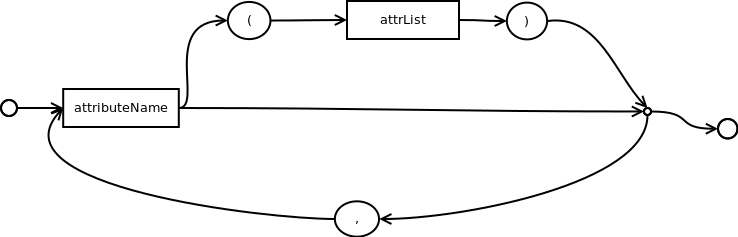
\includegraphics[scale=0.4]{images/attrList}
		\caption{Az \texttt{INSERT} szintaxis diagram \textit{attrList} komponense}
		\label{fig:attrListSytnax}
	\end{center}
\end{figure}

\begin{figure}[htb]
	\begin{center}
		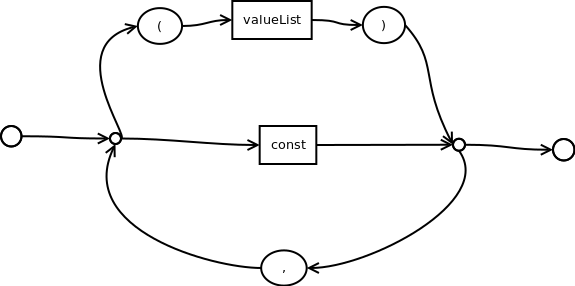
\includegraphics[scale=0.4]{images/valueList}
		\caption{Az \texttt{INSERT} szintaxis diagram \textit{valueList} komponense}
		\label{fig:valueListSytnax}
	\end{center}
\end{figure}

Ennek a lekérdezésnek az esetében is a builder objektum fában tárolja az objektumhoz tartozó attribútumokat. A kompozíció miatt, az attribútumok is tartalmazhatnak olyan attribútumokat, amelyek objektumok, így ezek között szülő-gyermek relációt lehet felfedezni, ezért a legegyszerűbb megoldásnak a fában való tárolás bizonyult.

\Aref{fig:insertTreeBuilder}. ábrán látható gráfokkal dolgozik az \texttt{INSERT} lekérdezés objektum. A jobb oldali gráf az, amelyre szüksége van a lekérdezés objektumnak, viszont ezt a nyelvi értelmező nem tudja előállítani, mivel az attribútumok és az értékek el vannak különítve egymástól a lekérdezésben. Látható, hogy a két baloldali gráfból előállítható az, amelyikre az \texttt{INSERT} objektumnak szüksége van, ezt viszont az \texttt{InsertBuilder} osztály a háttérben elvégzi.

\begin{figure}[htb]
	\begin{center}
		\includegraphics[scale=0.1]{images/InsertTreeBuilder}
		\caption{Az \texttt{INSERT} lekérdezés ábrázolása}
		\label{fig:insertTreeBuilder}
	\end{center}
\end{figure}

Az \texttt{InsertBuilder} a lekérdezésobjektum előállításához a háttérben két listát kezel. Az egyikben a séma megadása, tehát az attribútumokból felépíthető fa, míg a másikban az azonos szerkezetű, de már attribútum értékeket tartalmazó fa elemei szerepelnek.

Az \texttt{Insert} osztályon belül található egy \texttt{TreeBuilder} osztály, amely \texttt{TreeNode} csomópontokat tárol, és építi fel őket.
Amikor az \texttt{InsertBuilder} metódusai kívülről meghívódnak, ő az \texttt{Insert}-ből példányosított objektumnak közvetetten a \texttt{TreeBuilder} metódusait hívja tovább.

Az attribútum listában sorrendben tárolom az attribútumokat, illetve metaadatként azt, hogy a beszúrást követően a fában a szülő felé kell-e lépni, és ha igen, akkor hány szintet. \Aref{fig:insertTreeBuilder}. ábrán látható gráfok közül ez a lista a bal felső sarokban lévőt tárolja.

Az érték listában tárolom a \texttt{VALUES} kulcsszó után feltüntetett értékeket. \Aref{fig:insertTreeBuilder}. ábrán látható gráfok közül ez a lista a bal alsó sarokban lévőt tárolja.

\begin{comment}{Esetleg az ábrára is oda lehet írni, hogy melyik-melyik.}
\end{comment}

Az attribútum és az érték lista is egyaránt ugyan annyi elemet tárol, és ha mindkettőt feltöltötte a nyelvi feldolgozó, akkor az összeillesztésükhöz már csak egy iterációt kell megvalósítani, és a builder már attribútum-érték párokkal tud tovább dolgozni.

\subsection{DROP lekérdezés felépítése}

A \texttt{DROP} lekérdezéssel adatbázisokat, osztályokat és térképeket törölhetünk (\ref{fig:dropSytnax}. ábra). Ezt egy \texttt{DropBuilder} típusú objektum tudja lekérdezés objektummá átalakítani. Az átalakítás lépései kézenfekvő módon adódnak.

\begin{figure}[htb]
	\begin{center}
		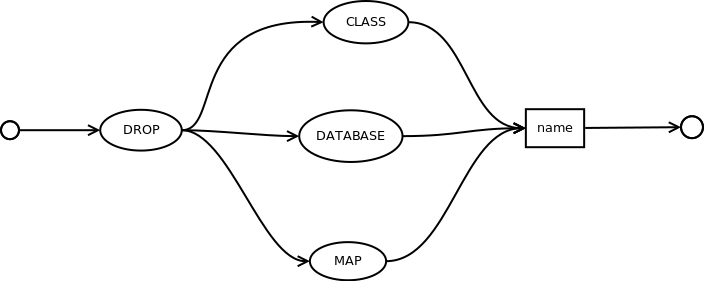
\includegraphics[scale=0.4]{images/drop}
		\caption{A DROP lekérdezés szintaxis diagramja}
		\label{fig:dropSytnax}
	\end{center}
\end{figure}

\section{Számítások optimalizálása}

Az adatbázismotor feladata levenni a terhet a felhasználó válláról,  optimalizált algoritmusokkal támogatni a lekérdezéseket. Térképfelosztás, pályaelem összevonás, ezek mind olyan feladatok, amelyek a térképműveletek gyorsabb végrehajtását idézik elő.

A dolgozat elsődleges célja a lekérdezőnyelv definiálása, és egy prototípus jellegű adatbázismotor implementálása. Az optimalizáció a későbbiekben nagyon fontos feladat, viszont egy olyan, nagyobb különálló témakörről van szó, amelynek bemutatása nem szerepel a dolgozat célkitűzései között.
